%%%%%%%%%%%%%%%%%%%%%%%%%%%%%%%%%%%%%%%%%%%%%%%%%%%%%%%%%%%%%%%%%%%%%%
% How to use writeLaTeX: 
%
% You edit the source code here on the left, and the preview on the
% right shows you the result within a few seconds.
%
% Bookmark this page and share the URL with your co-authors. They can
% edit at the same time!
%
% You can upload figures, bibliographies, custom classes and
% styles using the files menu.
%
%%%%%%%%%%%%%%%%%%%%%%%%%%%%%%%%%%%%%%%%%%%%%%%%%%%%%%%%%%%%%%%%%%%%%%

\documentclass[12pt]{article}

\usepackage{sbc-template}

\usepackage{graphicx,url}

%\usepackage[brazil]{babel}   
\usepackage[utf8]{inputenc} 

\usepackage{float}
\usepackage{hyperref}

\usepackage{listings}
\usepackage{color}

\definecolor{dkgreen}{rgb}{0,0.6,0}
\definecolor{gray}{rgb}{0.5,0.5,0.5}
\definecolor{mauve}{rgb}{0.58,0,0.82}

\lstset{frame=none,
  language=C++,
  aboveskip=3mm,
  belowskip=3mm,
  showstringspaces=false,
  columns=flexible,
  basicstyle={\small\ttfamily},
  numbers=none,
  numberstyle=\tiny\color{gray},
  keywordstyle=\color{blue},
  commentstyle=\color{dkgreen},
  stringstyle=\color{mauve},
  breaklines=true,
  breakatwhitespace=true,
  tabsize=3
}

     
\sloppy

\title{OTA}

\author{Fabricio Araújo Dias}

\address{Instituto Federal de Educação, Ciência e Tecnologia do Ceará
  (IFCE)\\
  Avenida Vice-Presidente José Alencar, S/N -- 61.939-140 -- Maracanaú -- CE -- Brasil
  \email{fabricio.araujo61@aluno.ifce.edu.br}
}

\begin{document} 

\maketitle

\begin{abstract}
    This report shows the step-by-step execution of the tenth practical activity of the Microcontrollers course, which consists of making updates to the ESP32 code without the need for a serial connection. The test was to send a code that turns an LED on and off.
\end{abstract}
     
\begin{resumo}
    Esse relatório mostra o passo a passo da realização da décima atividade prática da disciplina de Microcontroladores que consiste em fazer atualizações no código do ESP32 sem precisar de uma conexão serial. Testando enviando um código que acende e apaga um LED.
\end{resumo}

\section{Introdução}

A décima atividade prática da disciplina de Microcontroladores trabalha o uso de Over-The-Air (OTA) para o envio de atualizações do código no ESP32 sem o uso de um cabo serial. Ideal para resolver o problema de atualização quando o ESP32 não é de fácil acesso.

O envio do código é feito por uma página WEB e isso requer um certo conhecimento com o uso de HTML. De toda forma, a implementação foi bem simples, pois a questão é sobre o funcionamento do OTA.

Para realizar uma atualização como teste, foi criado um simples código para acender e apagar um LED com certa frequência.


\section{Configuração no ESP32}

O ESP32 utilizado na prática possui um LED interno. O que tornou desnecessária a utilização de protoboard, resistores e cabos.

\section{Desenvolvimento do Código}

Utilizamos a biblioteca Wifi e WifiClient para realizar a conexão à uma rede Wi-Fi, WebServer para criar um servidor Web, ESPmDNS para um multicast DNS e Update para a atualização.

\subsection{Conectando à rede Wi-Fi}

Começamos definindo constantes para que o SSID e a senha da rede Wi-Fi a qual o ESP32 irá se conectar.

\begin{lstlisting}
#define SSID ""
#define PASSWORD ""
\end{lstlisting}

Em \textit{setup}, inicialize o módulo Wi-Fi passando como parâmetros o SSID e a senha da rede. O fluxo entra num laço \textit{while} que irá executar até o método \textit{status} do módulo Wi-Fi retorne um valor que afirme que a conexão foi realizada. Colocamos um \textit{delay} de meio segundo dentro do \textit{while}.

\begin{lstlisting}
WiFi.begin(SSID, PASSWORD);

while (WiFi.status() != WL_CONNECTED) {
    delay(500);
    Serial.print(".");
}
\end{lstlisting}

Ele sairá do laço quando a conexão estiver concluída.

\begin{lstlisting}
Serial.println("");
Serial.println("Connected to Wi-Fi.");
\end{lstlisting}

\subsection{Definindo um endereço mDNS}

Inicializamos um servidor DNS multicast para que não seja preciso utilizar endereços IPs dinâmicos para acessar nossa página WEB.

Definimos uma constante para guardar o hostname. O nome escolhido foi "esp32" que, mesmo sendo comum, pode ser usado porque ele só vai funcionar na rede local.

\begin{lstlisting}
#define HOSTNAME "esp32"
\end{lstlisting}

Para inicializar o servidor, utilizamos o método \textit{begin} do módulo \textit{mDNS} e passamos como parâmetro o nome do \textit{host} que escolhemos anteriormente. O método retorna um valor que mostra se o servidor foi inicializado ou não. Se ele não inicializou, usamos \textit{ESP.restart()} para reiniciar o ESP32.

\begin{lstlisting}
if (!MDNS.begin(HOSTNAME)) { 
    Serial.println("Error setting up MDNS responder!");
    delay(1000);
    ESP.restart();        
}
\end{lstlisting}

Se ele foi inicializado, então poderemos acessar a nossa página WEB pelo endereço \textit{http://esp32.local}.

\subsection{Desenvolvendo as páginas WEB}

Para criar páginas WEB, precisamos codificar em HTML, mas isso foi feito dentro do código em C++. O código em HTML foi armazenado em \textit{const char *} e cada linha do código foi colocado entre àspas duplas.

Para criamos uma variável chamada \textit{server} da classe \textit{WebServer} para que tenhamos um servidor WEB com o qual iremos utilizá-lo para a comunicação com o ESP32. Ele inicializa junto com um número de porta. Escolhemos a porta 80.

\begin{lstlisting}
WebServer server(80);
\end{lstlisting}

\subsubsection{Escrevendo o código HTML}

Começando pela página de \textit{login}, criamos um formulário simples que pega um \textit{username} e uma senha. Usamos a tag \textit{form} para criar o formulário e a tag \textit{table} para dispor os elementos do formulário. A tag \textit{input} guarda as informações que o usuário fornece. Também usamos essa tag para criar um botão que servirá de gatilho.

\begin{lstlisting}
"<form name="loginForm">"
    "<label>Login:</label>"
    "<input type="text" name="userid"/>"

    "<label>Senha:</label>"
    "<input type="password" name="pwd"/>"

    "<input type="submit" onclick='check(this.form)'" "value="Identificar"/>"
"</form>"
\end{lstlisting}

O \textit{script} da página é feito em JavaScript. Nessa página, ele possui uma função chamada check e confere as credenciais. Como não é um projeto de verdade, se o \textit{username} e a senha forem iguais à "admin", a página redireciona para a página \textit{serverIndex}.

\begin{lstlisting}
"function check(form) {"
    "if(form.userid.value=='admin' && form.pwd.value=='admin')"
    "{"
        "window.open('/serverIndex')"
    "} else {"
        alert('Error Password or Username')
    "}"
"}"
\end{lstlisting}

Para a página \textit{serverIndex}, temos um formulário para o envio de um código binário para o ESP32.

Para começar, importante a biblioteca \textit{jQuery} para que possamos fazer requisições assíncronas com o Ajax.

\begin{lstlisting}
"<script src=
'https://ajax.googleapis.com/ajax/libs/jquery/3.2.1/jquery.min.js'>
</script>"
\end{lstlisting}

Criamos o formulário que possui um \textit{input} que recebe um arquivo e outro \textit{input} de \textit{submit}.

\begin{lstlisting}
"<form method='POST' action='#' enctype='multipart/form-data' id='upload_form'>"
    "<input type='file' name='update'>"
    "<input type='submit' value='Update'>"
"</form>"
 "<div id='prg'>Progress: 0%</div>"
\end{lstlisting}

No script, existe uma função que é executada quando o usuário pressiona o botão de \textit{submit}. 

\begin{lstlisting}
$('form').submit(function(e){
    e.preventDefault();
\end{lstlisting}

Acessamos o formulário pela \textit{ID} e transformamos os dados no objeto FormData.

\begin{lstlisting}
var form = $('#upload_form')[0];
var data = new FormData(form);
\end{lstlisting}

Configuramos a requisição Ajax que será do tipo POST e irá para \textit{/update}. Passamos os dados no campo \textit{data}. Deixamos os campos \textit{contentType} e \textit{processData} em \textit{false} para que não ocorra alterações no arquivo.

\begin{lstlisting}
$.ajax({
    url: '/update',
    type: 'POST',
    data: data,
    contentType: false,
    processData: false,
    xhr: function() { ... },
    success: function(d, s) {
        "console.log('Success!')"
    },
    error: function (a, b, c) {
        "console.log('Fail!')"
    }
});
\end{lstlisting}

O campo \textit{xhr} significa \textit{XMLHttpRequest} que é um objeto que fornece a funcionalidade de recuperar dados de uma URL sem precisar atualizar a página inteira. Nesse caso, ele atualiza o progresso de envio que é exibidio na página.

\begin{lstlisting}
xhr: function() {
    var xhr = new window.XMLHttpRequest();
    xhr.upload.addEventListener('progress', function(evt) {
        if (evt.lengthComputable) {
            var per = evt.loaded / evt.total;
            $('#prg').html('Progresso: ' + Math.round(per*100) + '%');
        }
    }, false);
    return xhr;
}
\end{lstlisting}

\subsubsection{Configurando as páginas}

Essa parte é feita em \textit{setup}. Para configurar as páginas WEB, vamos utilizar o método \textit{on} da classe \textit{WebServer}. Ela recebe como parâmetros o endereço da página, o método HTTP e uma função que é executada. Na função, enviamos um header com o método \textit{sendHeader} e também enviamos o código HTML utilizando o método \textit{send}. O método \textit{send} recebe um código de status de resposta HTTP, o tipo do conteúdo e o conteúdo em si.

Essa é a parte do código onde configuramos a página de login.
\begin{lstlisting}
server.on("/", HTTP_GET, []() {
    server.sendHeader("Connection", "close");
    server.send(200, "text/html", loginIndex);
});
\end{lstlisting}

Fazemos a mesma coisa com a página \textit{serverIndex}.

\begin{lstlisting}
server.on("/serverIndex", HTTP_GET, []() {
    server.sendHeader("Connection", "close");
    server.send(200, "text/html", serverIndex);
});
\end{lstlisting}

Agora, configuramos a página de envio do arquivo para o ESP32. Como foi mostrado ao se implementar o código HTML, o arquivo será enviado para \textit{/update}. Diferente da outras duas páginas que criamos, o método HTTP dessa página é POST.

\begin{lstlisting}
server.on("/update", HTTP_POST, []() {
    server.sendHeader("Connection", "close");
    server.send(200, "text/plain", (Update.hasError()) ? "FAIL" : "OK");
    ESP.restart();
}, []() { ... }
\end{lstlisting}

O método \textit{on} é sobrecarregado e pode recebe mais até duas funções, que é o ideal para enviar arquivos. Nessa função, utilizamos o método \textit{upload} de \textit{server} para que ele retorne os dados do \textit{upload} que está sendo realizado. Assim, executamos códigos diferentes em cada momento do envio.

\begin{lstlisting}
HTTPUpload& upload = server.upload();
\end{lstlisting}

A variável \textit{upload} é uma \textit{struct}, e ela possui uma variável \textit{status} que informa qual o status do envio.

\begin{lstlisting}
upload.status
\end{lstlisting}

Se o \textit{status} for \textit{UPLOAD\_FILE\_START}, quer dizer que o \textit{upload} está para iniciar. Por isso, utilizamos o método begin da classe Upload para conferir se há espaço disponível no ESP32 para realizar a atualização. Como o tamanho do arquivo é indefinido, passamos \textit{UPDATE\_SIZE\_UNKNOWN}.

\begin{lstlisting}
if (upload.status == UPLOAD_FILE_START) {
    Serial.printf("Update: %s\n", upload.filename.c_str());
    if (!Update.begin(UPDATE_SIZE_UNKNOWN)) 
        Update.printError(Serial);
} 
\end{lstlisting}

Se o status for \textit{UPLOAD\_FILE\_WRITE}, então vamos usar o método write da classe \textit{Upload} para escrever o que está guardado no buffer na memória flash do ESP32. Passamos também o tamanho do buffer na chamada do método. Essas informações estão guardadas nas variáveis \textit{buf} e \textit{currentSize} da struct \textit{upload}.

\begin{lstlisting}
if (upload.status == UPLOAD_FILE_WRITE) {
    if (Update.write(upload.buf, upload.currentSize) != upload.currentSize) 
        Update.printError(Serial);
}
\end{lstlisting}

E por último, se status for \textit{UPLOAD\_FILE\_END}, usamos o método \textit{end} da classe Upload que retorna um booleano se toda a escrita foi realizada com sucesso. Esse método recebe como parâmetro um booleano para definir se ter restado dados a serem enviados influenciará na resposta ou não.

\begin{lstlisting}
if (upload.status == UPLOAD_FILE_END) {
    if (Update.end(true))             
        Serial.println("The writing was a success!");
    else
        Update.printError(Serial);
} 
\end{lstlisting}

Terminada a configuração das páginas, só resta utilizar o método \textit{begin} do \textit{WebServer} para iniciar o servidor WEB.

\begin{lstlisting}
server.begin();
\end{lstlisting}

Por fim, em \textit{loop}, colocamos para executar o método \textit{handleClient} para que fique fazendo as chamadas das funções que acabamos de criar. Colocamos um pequeno \textit{delay}.

\begin{lstlisting}
void loop() {
    server.handleClient();
    delay(1);
}
\end{lstlisting}

\section{Envio do código e teste}

Conectando o ESP32 ao computador e enviando o código que criamos para ele, podemos acessar a página WEB acessando \textit{esp32.local} em qualquer navegador, desde que estejam na mesma rede.

Como foi especificado quando escrevemos o código em HTML, o \textit{username} e a senha são "admin".

\begin{figure}[H]
    \centering
    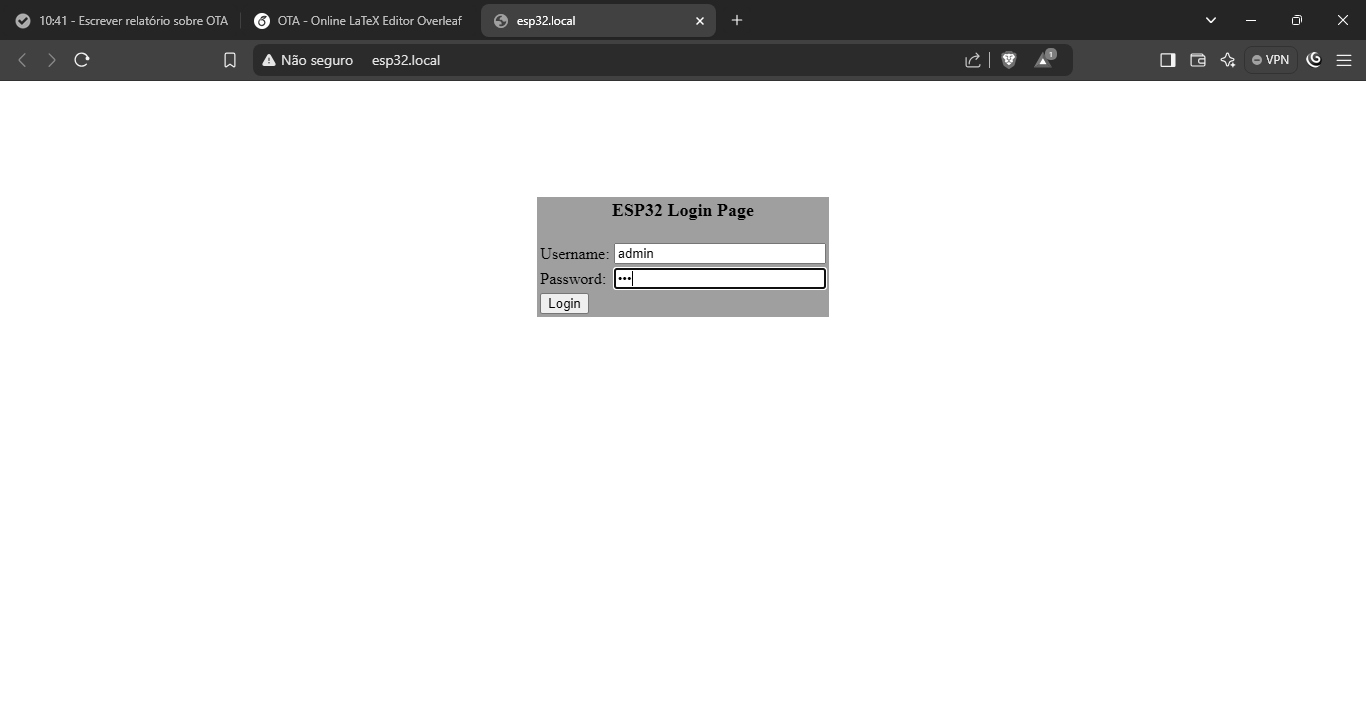
\includegraphics[width=0.5\linewidth]{img/Captura de tela 2024-12-05 194630.jpg}
    \caption{Página de login.}
    \label{fig:loginIndex}
\end{figure}

Ao entrar na página de envio, podemos selecionar algum arquivo do nosso computador para enviar para o ESP32. O arquivo precisa ser um binário.

\begin{figure}[H]
    \centering
    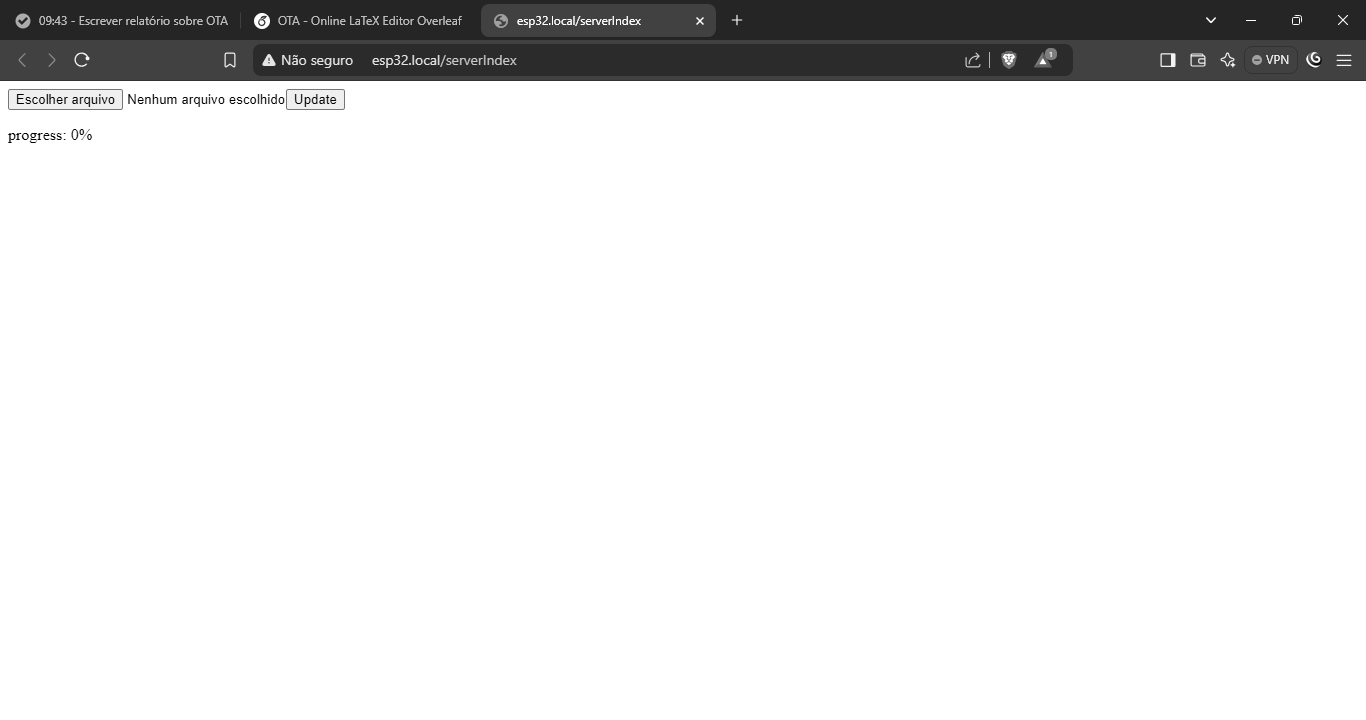
\includegraphics[width=0.5\linewidth]{img/Captura de tela 2024-12-05 194720.jpg}
    \caption{Página de envio de arquivo.}
    \label{fig:serverIndex}
\end{figure}

Para testar, criamos um pequeno código para acender e apagar um LED. Então, voltamos ao código e adicionamos esses trechos ao código que já criamos.

\begin{lstlisting}
// ...
#define RED 19
// ...
void setup() {
    // ...
    pinMode(RED, OUTPUT);
}

void loop() {
    // ....
    digitalWrite(RED, HIGH);
    delay(2000);
    digitalWrite(RED, LOW);
    delay(2000);
}
\end{lstlisting}

Feito essa atualização no código, não iremos fazer \textit{upload}. Faremos apenas \textit{build} usando o comando \textit{Ctrl + Alt + B}.

Na pasta do projeto no VSCode, acessamos o endereço $.pio \backslash build \backslash esp32dev$ e copiamos e salvamos o arquivo \textit{firmware.bin}, pois esse é o nosso código convertido em binário.

Retornando à página WEB, selecionamos o \textit{firmware.bin} e apertamos o botão \textit{enviar}. Após a porcentagem ter chegado à 100\%, o código foi enviado e é possível ver o resultado da atualização.

\begin{figure}[H]
    \centering
    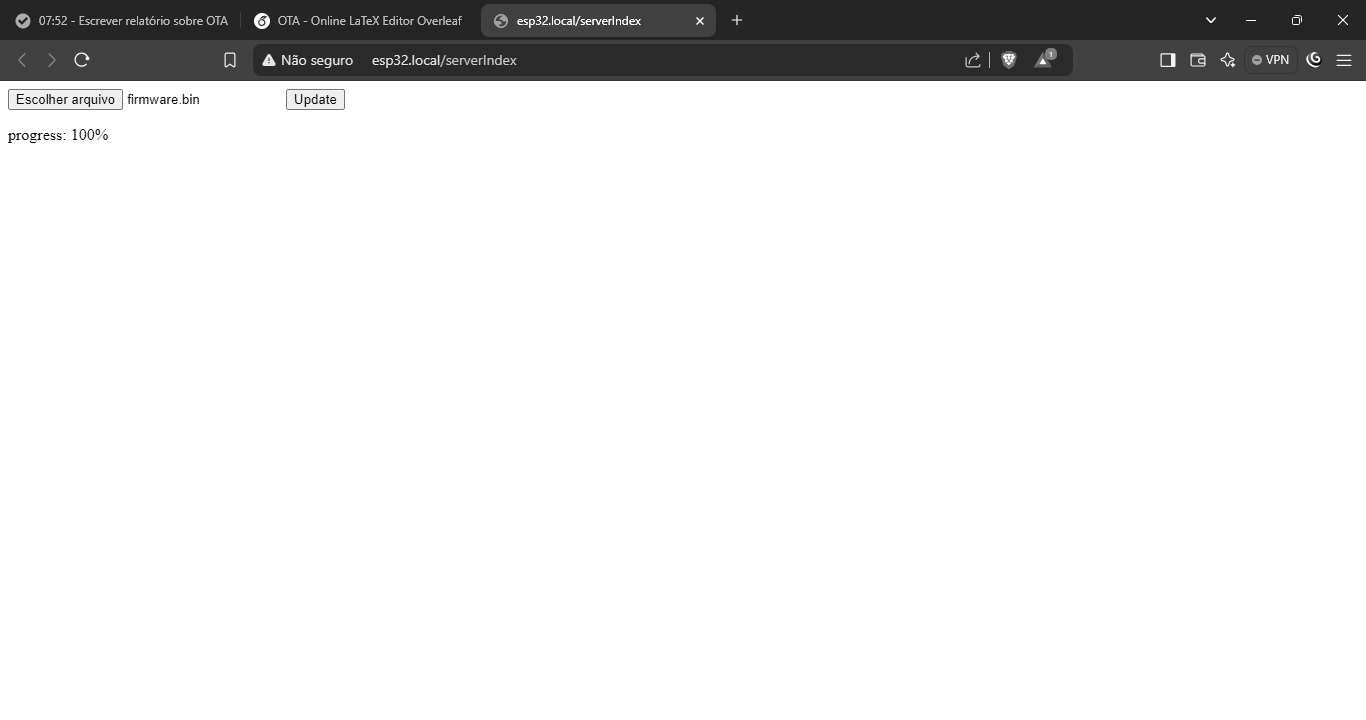
\includegraphics[width=0.5\linewidth]{img/Captura de tela 2024-12-05 194905.jpg}
    \caption{Enviando arquivo.}
    \label{fig:sending}
\end{figure}

\section{Considerações Finais}

Algumas partes do código foram simplicadas para se disporem no relatório. As mudanças foram mínimas. O código completo pode ser conferido nesse \href{https://github.com/fabricio-araujo94/microcontroladores/tree/main/ota_}{repositório no GitHub}.

Um vídeo com a execução da prática no laboratório pode ser conferido nesse \href{https://youtube.com/shorts/Of_eVqhS5-g?feature=share}{link}.

\end{document}